\documentclass{csafedoc}
\usepackage{algorithmic} % to explain any algorithms you might have
\usepackage{listings} % in case you want to drop in some R code
\usepackage{bm}

\begin{document}

\title{ShoeComp}
\author{CSAFE}
\date{\today}

\begin{titlingpage}
	\begin{vplace}
		\vfill{}
		\begin{center}
			\begin{tabular}{cl}
				\raisebox{-.35\height}[0pt][0pt]{
\includegraphics[height=55pt]{images/shoecomp-logo.png}} & {\fontsize{40}{35}\selectfont\bfseries\textcolor{pantone654c}{shoecomp}} \\
					 & {\fontsize{21}{21}\selectfont\bfseries\textcolor{pantone637c}{USER GUIDE}}
			\end{tabular}
			\par
			\vspace*{25pt}
			\textcolor{pantone654c}{\rule{0.85\textwidth}{2pt}}
			\par
			\vspace*{20pt}
			\begin{tabular}{c!{\color{pantone425c}\vrule}c}
				
\includegraphics[height=1cm,keepaspectratio]{images/csafe-logo.png} &
            
\includegraphics[height=1cm,keepaspectratio]{images/csafe-tools-logo.png}
		    \end{tabular}
		\end{center}
		\vfill{}
	\end{vplace}
		\hfill{}
		\textbf{\textcolor{pantone654c}{Last Modified: \today}}
\end{titlingpage}
\newpage

\chapter{Introduction}%
\label{sec:intro}

This document provides a user guide for ShoeComp, a software tool for the markup and
alignment of shoeprint images. ShoeComp is developed by CSAFE, the Center for Statistics
and Applications in Forensic Evidence at Iowa State University. It is part of the CSAFE
Tools collection, and aims to provide a graphical user interface for annotating, aligning,
and comparing shoeprint images. ShoeComp aims to provide the following features:

\begin{itemize}
	\item mark interest points on footwear impression images
	\item align footwear impressions using marked interest points, removing differences in
	      rotation, translation, and scale between the images -- by difference in scale, we
	      refer to a missing L-scale in the image or if it is unclear how the physical size of the
	      shoeprint translates to a length in pixels.
	\item compare aligned images to produce similarity scores -- we currently provide an
	      example similarity score to showcase how scores for such comparisons might be presented.
	\item view similarity scores in context of reference distributions -- the provided reference
	      distribution is based on an experiment run on data from \cite{soyoung}, and are
	      not representative.
	\item save interest point markups and alignments for reports or future comparisons with other metrics
\end{itemize}

ShoeComp implements a generalized version of the maximum clique alignment algorithms
described in \cite{soyoung, gvs1} to align the shoeprint images. ShoeComp is written in
the \texttt{Java} programming language as a plugin for
\rref{ImageJ/FIJI}{https://imagej.net/software/fiji/}, a popular open-source image processing and
annotation tool. It also uses ImageJ's \rref{Action
	Bar}{https://imagej.net/plugins/action-bar} plugin to provide a simple user interface. The
source code of ShoeComp is publicly available at:

\begin{center}
	\selfref{https://github.com/CSAFE-ISU/shoecomp}
\end{center}

where you can also download the latest built version from the
\rref{Releases}{https://github.com/CSAFE-ISU/shoecomp/releases} page. Below is a
screenshot of the basic ShoeComp user interface:

\begin{figure}[htbp]
	\begin{center}
		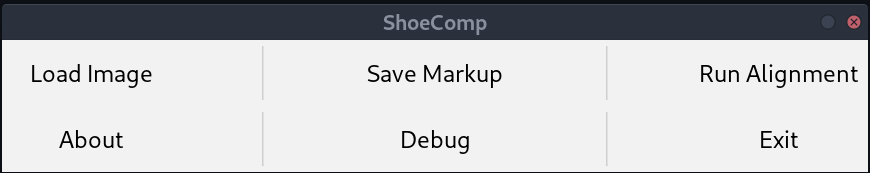
\includegraphics[height=0.4\linewidth]{images/shoecomp.png}
	\end{center}
	\caption{The basic Graphical User Interface (GUI) of ShoeComp. There are six options:
		\texttt{Load Image} to load a new shoeprint image or resume previous markup work, \texttt{Save
			Markup} to save markup work for export or later use, \texttt{Run Alignment} to align two
		shoeprint images, \texttt{About} displays information about ShoeComp and CSAFE,
		\texttt{Settings} toggles the classic ImageJ GUI for advanced usage or debugging, and
		\texttt{Exit} closes the application.}
	\label{fig:shoecomp_base}
\end{figure}

ShoeComp is designed in a manner similar to that of
\rref{FRSTAT}{https://zenodo.org/records/4426484}, which is a tool for the statistical
interpretation of friction ridge skin impression evidence. However, we note that ShoeComp
at present \underline{does not} provide any statistical analysis or interpretation
capabilities, the scores and reference distributions are illustrative examples for how
such things could be done.

\newpage
\chapter{User Guide}%
\label{sec:userguide}

Let's go through the basic steps to mark and align shoeprint images using ShoeComp. As an
example for this guide, we will be using images from the FBI Boots Dataset \cite{boots}, available
publicly at

\begin{center}
	\selfref{https://doi.org/10.17605/OSF.IO/EV8MK}.
\end{center}

We will be using the following two images:

\begin{itemize}
	\item \texttt{QK010-QC.JPG} as our questioned image, and
	\item \texttt{QK010-KF.JPG} as our reference image.
\end{itemize}

You can download the images from \selfref{https://doi.org/10.17605/OSF.IO/EV8MK}
(available in `JPEG Images Part 1 of 4'), but if this is your first time trying ShoeComp,
we recommend downloading our example markups from
\selfref{https://github.com/CSAFE-ISU/releases}, the same link where this manual is
available.

\section{Downloading ShoeComp}

You can download ShoeComp as a ZIP file from
\selfref{https://github.com/CSAFE-ISU/releases}. Select the latest version, and download
the ZIP file according to your operating system. For this guide we will be using a Windows
computer.

\begin{figure}[htbp]
	\begin{center}
		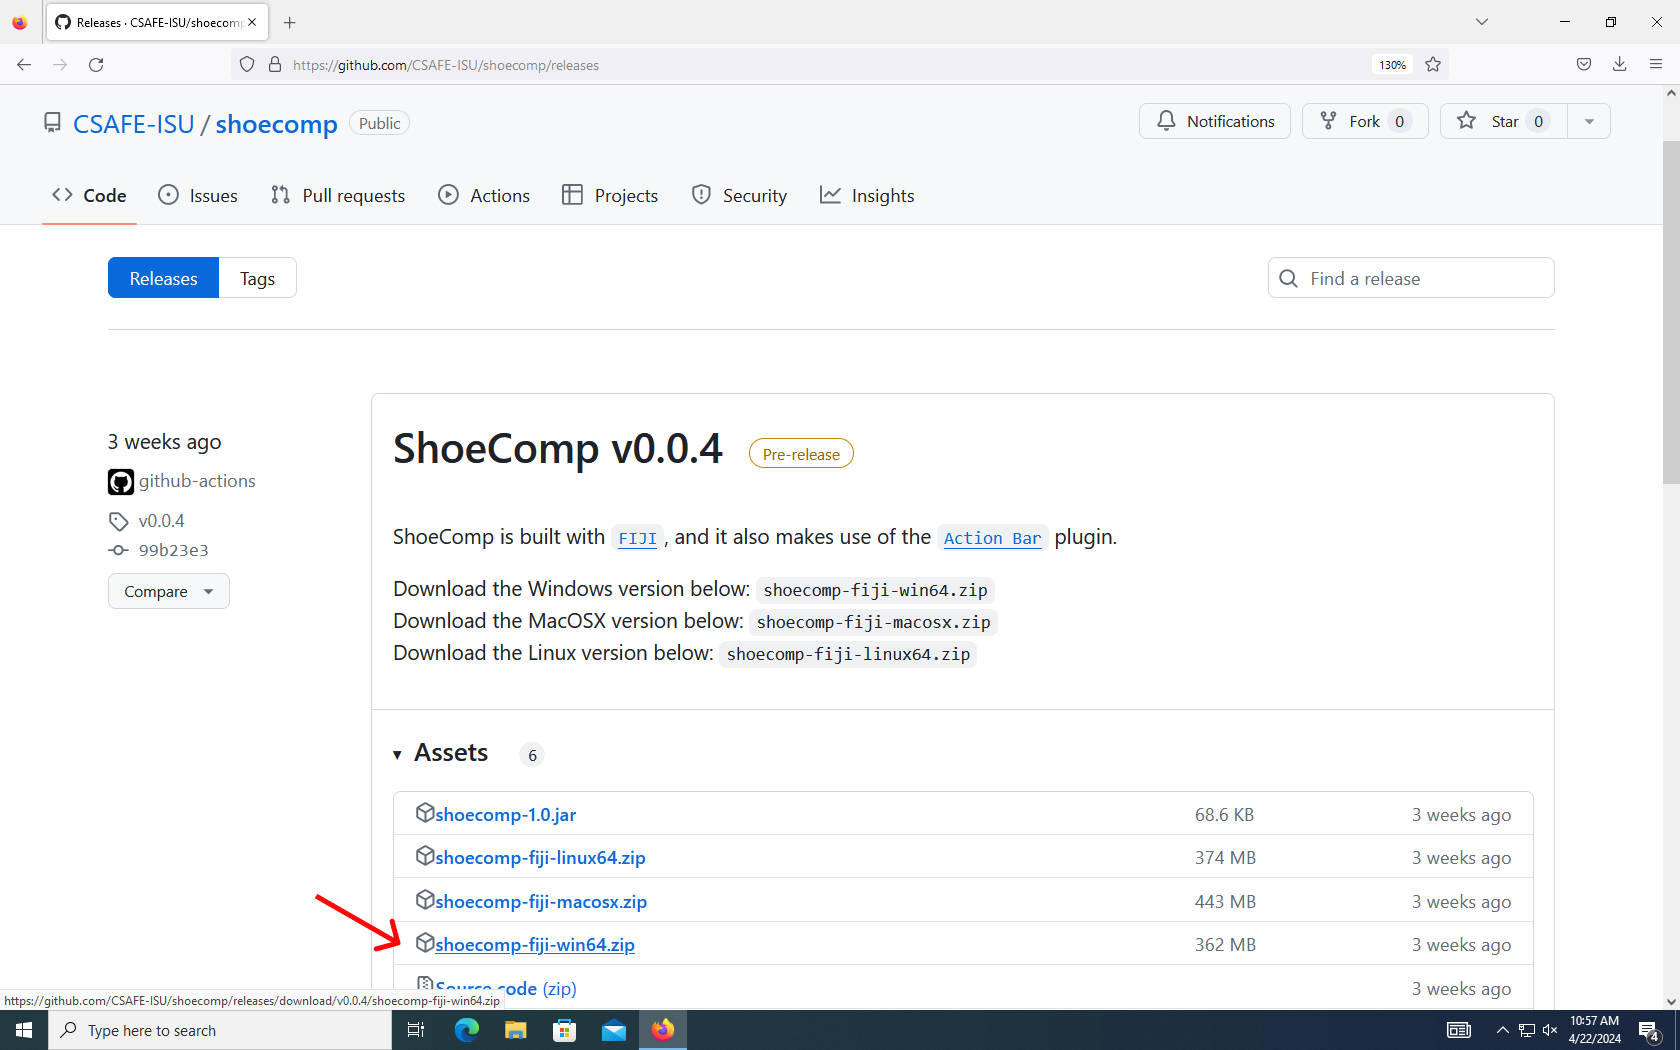
\includegraphics[width=0.8\linewidth]{images/step_1-anno.png}
	\end{center}
	\caption{Download the latest version of ShoeComp as a ZIP File from the CSAFE-ISU Github page.}
	\label{fig:step1}
\end{figure}

\section{Installing ShoeComp}

ShoeComp does not require any installation on Windows or Linux, you can just unzip the ZIP
file and it is ready to use:

\begin{figure}[H]
	\begin{center}
		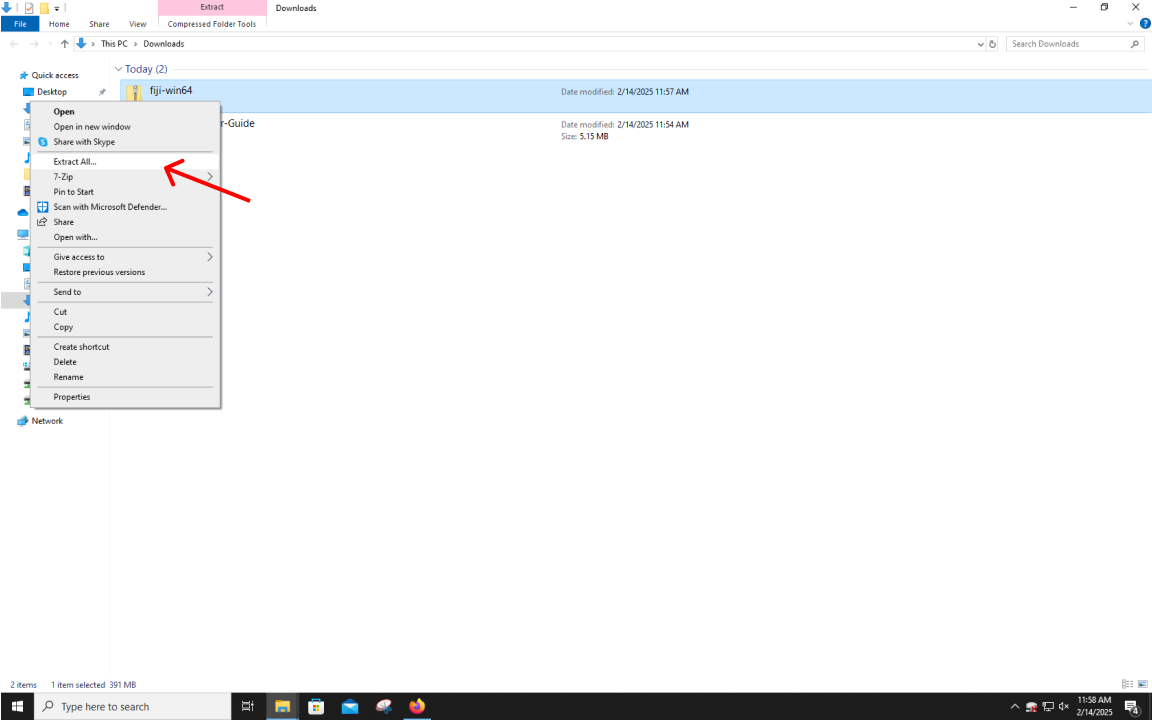
\includegraphics[width=0.8\linewidth]{images/step_2-anno.png}
	\end{center}
	\caption{Installing ShoeComp. Just unzip the ZIP file and you're ready!}
	\label{fig:step2}
\end{figure}

On MacOS, you may not need to unzip, but you will need to access Settings to allow the
\texttt{FIJI} application to run. After unzipping, you should find the \texttt{Fiji.app}
folder and find the \texttt{ImageJ} application to double-click:

\begin{figure}[H]
	\begin{center}
		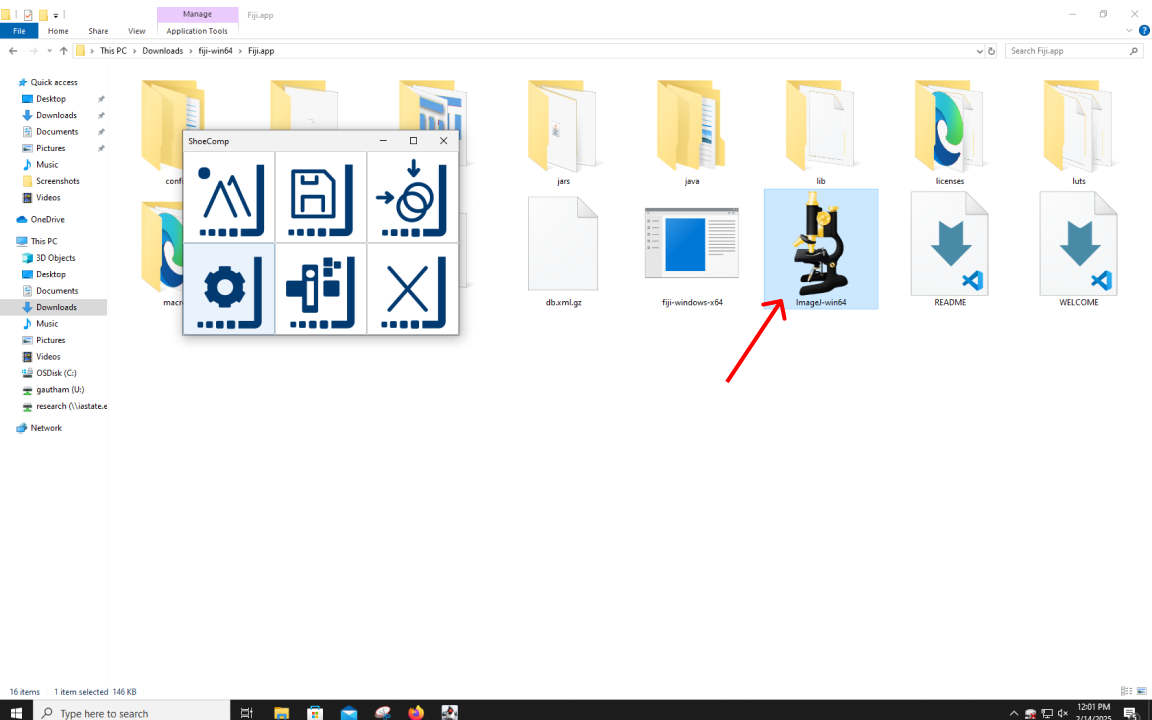
\includegraphics[width=0.8\linewidth]{images/step_3-anno.png}
	\end{center}
	\caption{ShoeComp is built as a plugin for FIJI/ImageJ. Double-click on the ImageJ application to start
		ShoeComp.}
	\label{fig:step3}
\end{figure}

\section{Loading an Image}

After opening the ShoeComp GUI, we need to load images. Click on the \texttt{Load Image}
button, select \texttt{Load Image} again, and then select the image file to read:

\begin{figure}[H]
	\begin{center}
		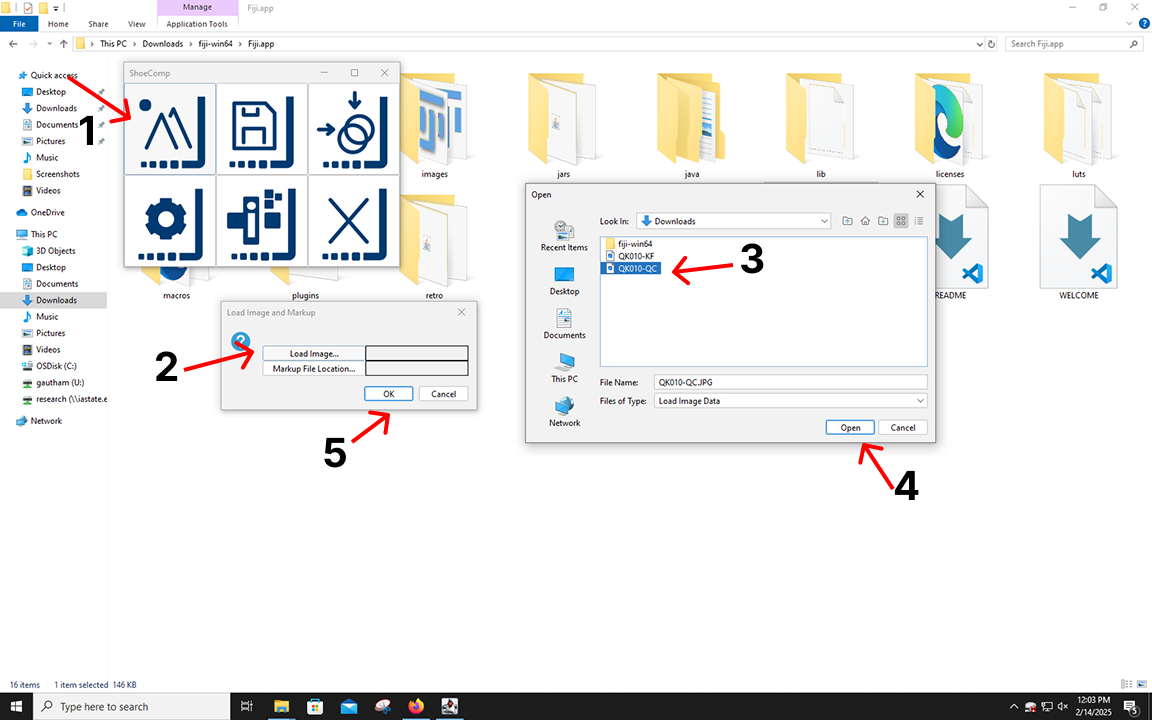
\includegraphics[width=0.8\linewidth]{images/step_4a-anno.png}
	\end{center}
	\caption{Loading an image into ShoeComp: Click on \texttt{Load Image}, Click on
		\texttt{Load Image} again, Select the image file, Click on \texttt{Open}, Click on \texttt{OK}.}
	\label{fig:step4a}
\end{figure}

After loading the image, you will first need to mark \underline{the relevant area of the
	shoeprint}. A window will appear next to the image, which you can close after marking a
polygon bounding the relevant area of the shoeprint.

\begin{figure}[H]
	\begin{center}
		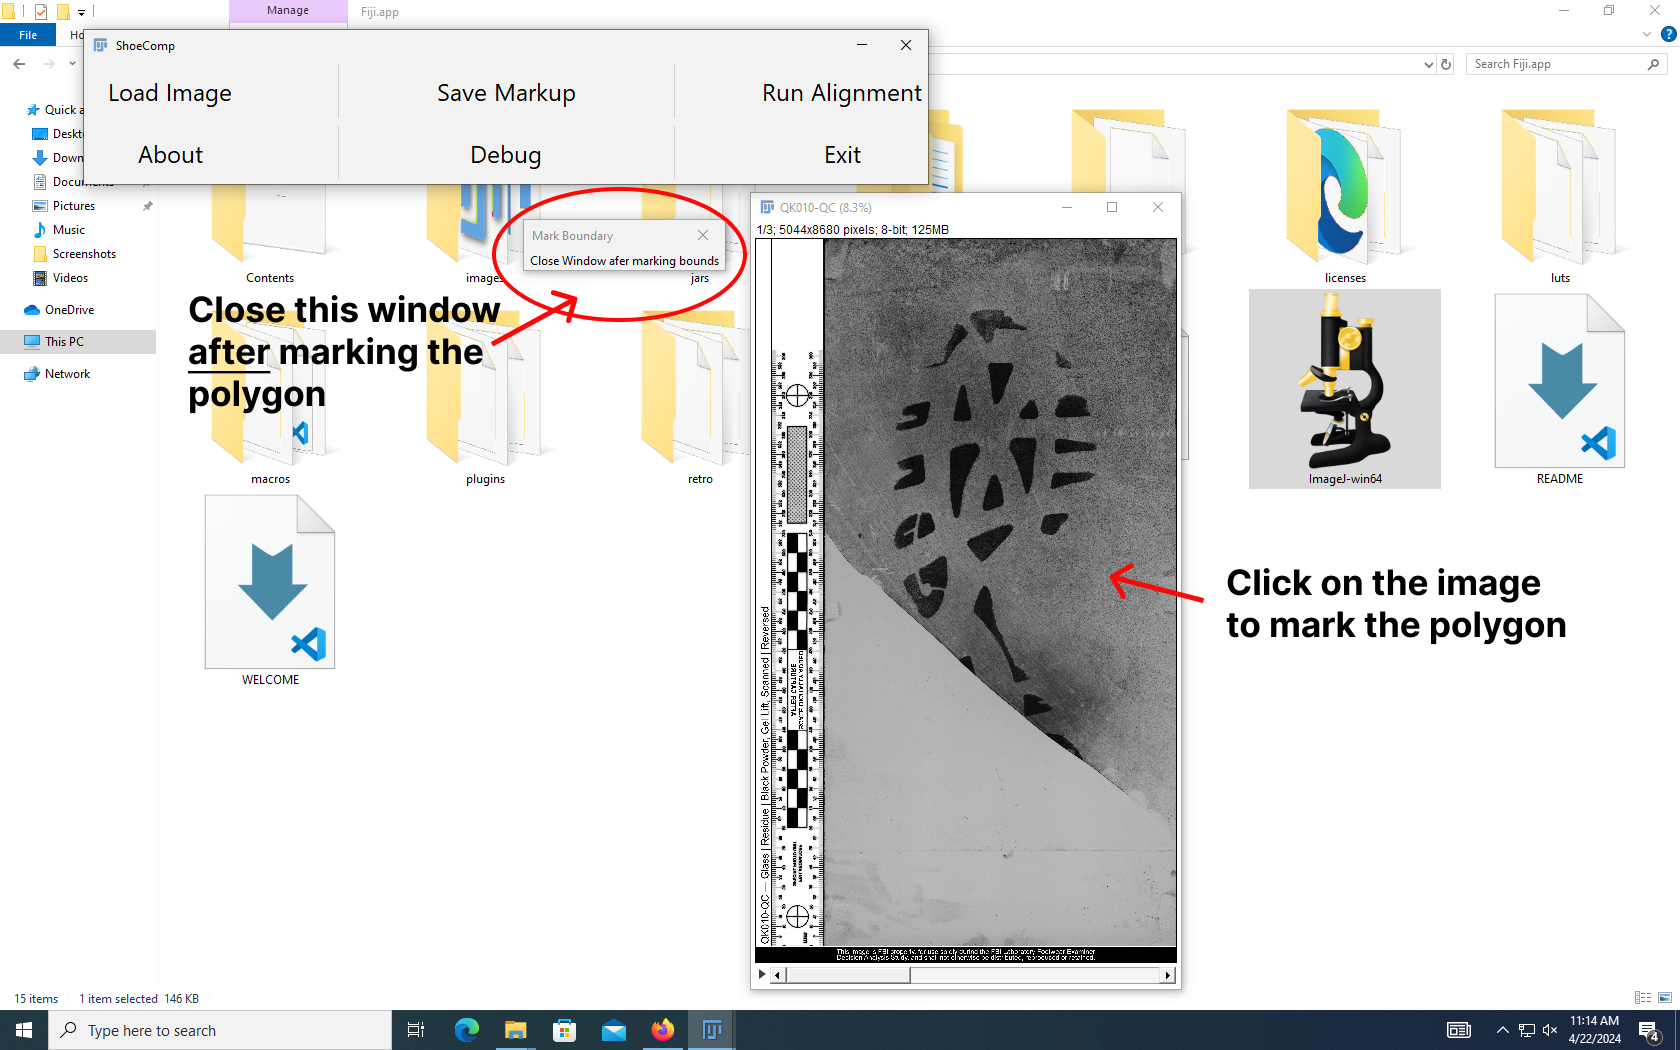
\includegraphics[width=0.8\linewidth]{images/step_4b-anno.png}
	\end{center}
	\caption{Start marking the boundary polygon. Click on the image to mark the boundary.
		Don't close the window before completing the polygon!}
	\label{fig:step4b}
\end{figure}

Once you've marked the boundary polygon, you can close that window so you can focus on
marking interest points in the relevant area of the shoeprint.

\begin{figure}[H]
	\begin{center}
		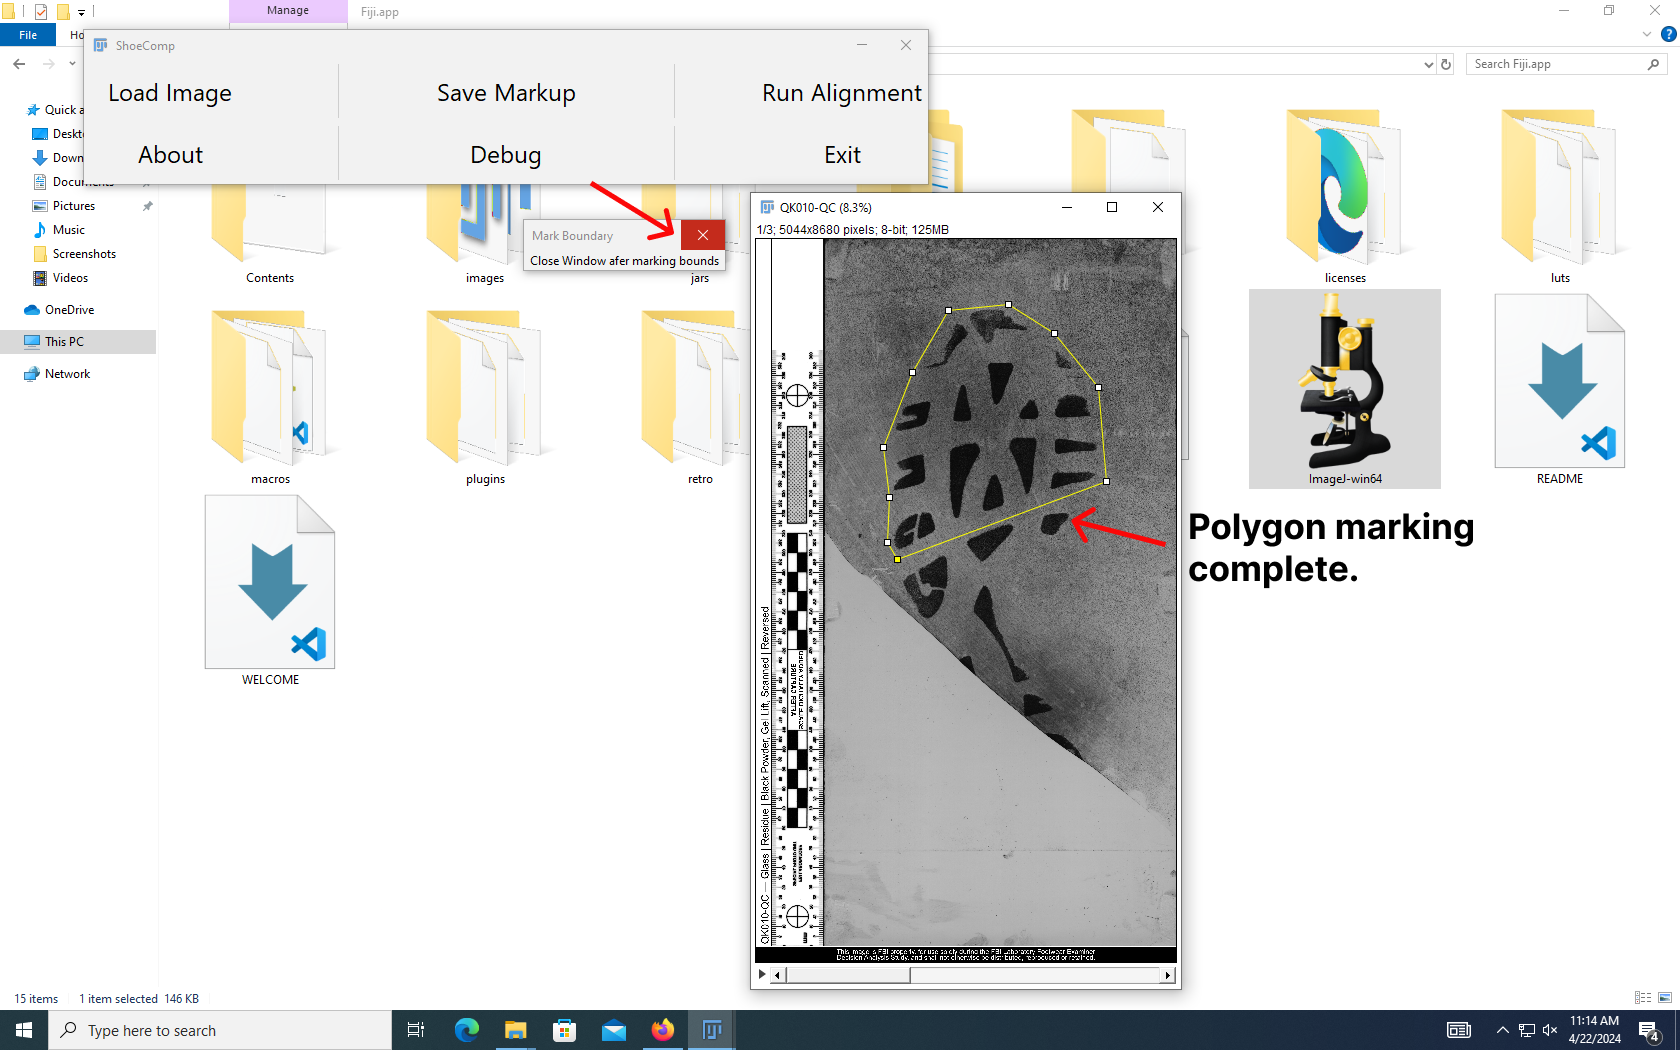
\includegraphics[width=0.8\linewidth]{images/step_4c-anno.png}
	\end{center}
	\caption{The boundary polygon has been marked, so now we can click this button.}
	\label{fig:step4c}
\end{figure}

Mark interest points by clicking on the image. We usually use corners of geometric shapes,
but you can use any points that can be marked consistently (like centers of circles). If
you want to mark the points with a bit more accuracy, you can use \texttt{Ctrl+Scroll} or
the \texttt{+} key to zoom the image at the location of the mouse. If you've marked a
point wrongly or have too many points marked, use \texttt{Alt+Click} to remove a marked
point.

\begin{figure}[H]
	\begin{center}
		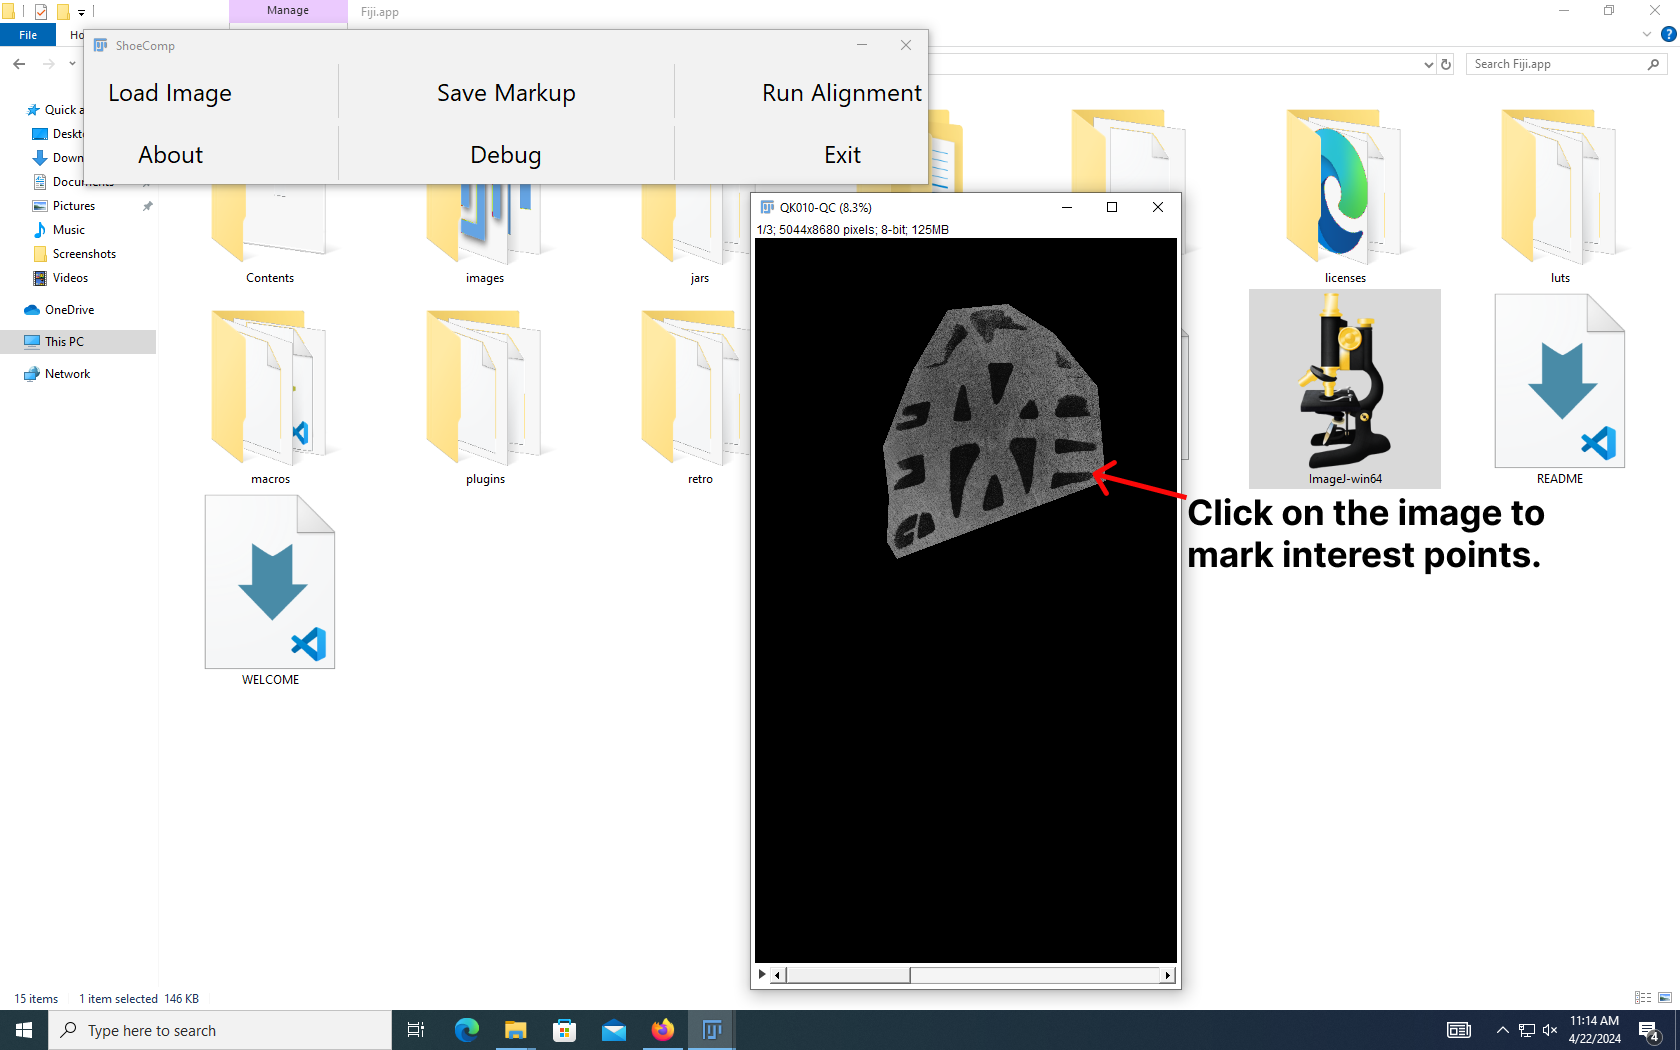
\includegraphics[width=0.8\linewidth]{images/step_4d-anno.png}
	\end{center}
	\caption{Mark interest points by clicking. Use \texttt{Ctrl+Scroll} or the \texttt{+} key
		to zoom the image at the location of the mouse, and \texttt{Alt+Click} to remove a marked
		point. If you just scroll by mistake, you will see the polygon mask and original image, so
		scroll back to the markup.}
	\label{fig:step4d}
\end{figure}

Theoretically, we only need 3 points for solving rotation, translation, and scale,
but there might be noise in the image, non-linear distortions, and marking error, so
\underline{20-30 marked points} is a rule of thumb for alignment.

\begin{figure}[H]
	\begin{center}
		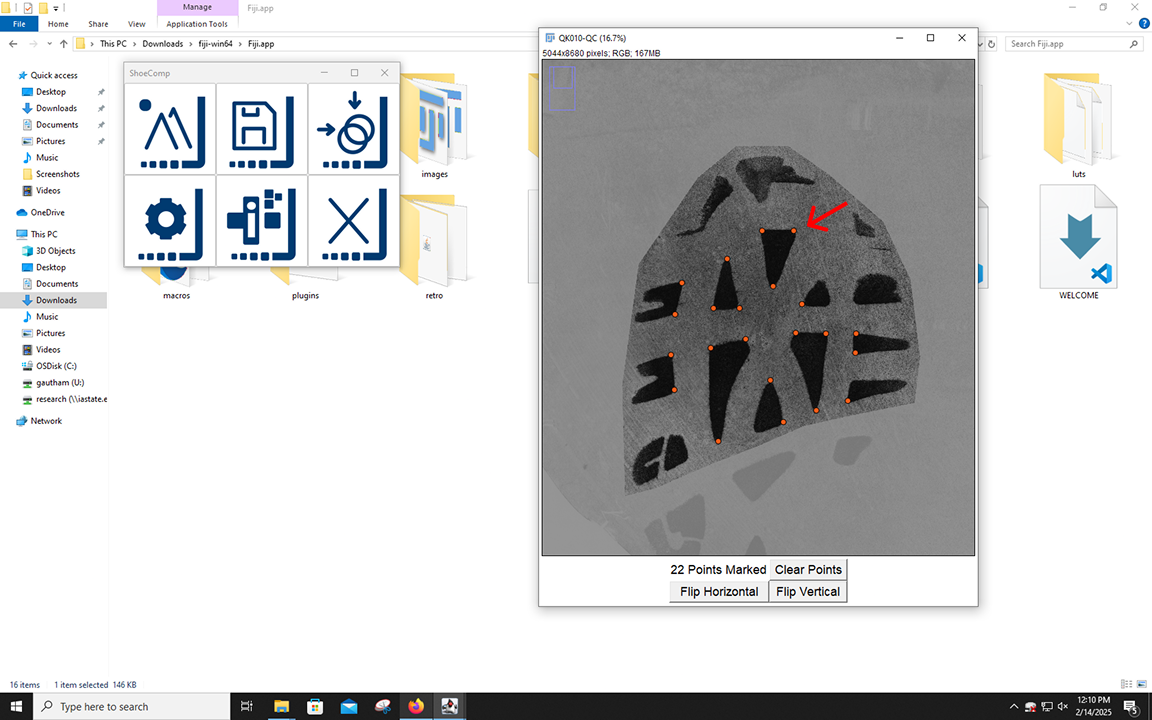
\includegraphics[width=0.8\linewidth]{images/step_4e-anno.png}
	\end{center}
	\caption{A few interest points have been marked on the image.}
	\label{fig:step4e}
\end{figure}

\section{Saving/Reloading Markup}

After you've marked the relevant area as polygon and some interest points, you might want
to save your markup to export to other tools and resume at a later point. Click on
\texttt{Save Markup}, and select file locations for saving the markup. The markup is saved
as a text file in the JSON format.

\begin{figure}[H]
	\begin{center}
		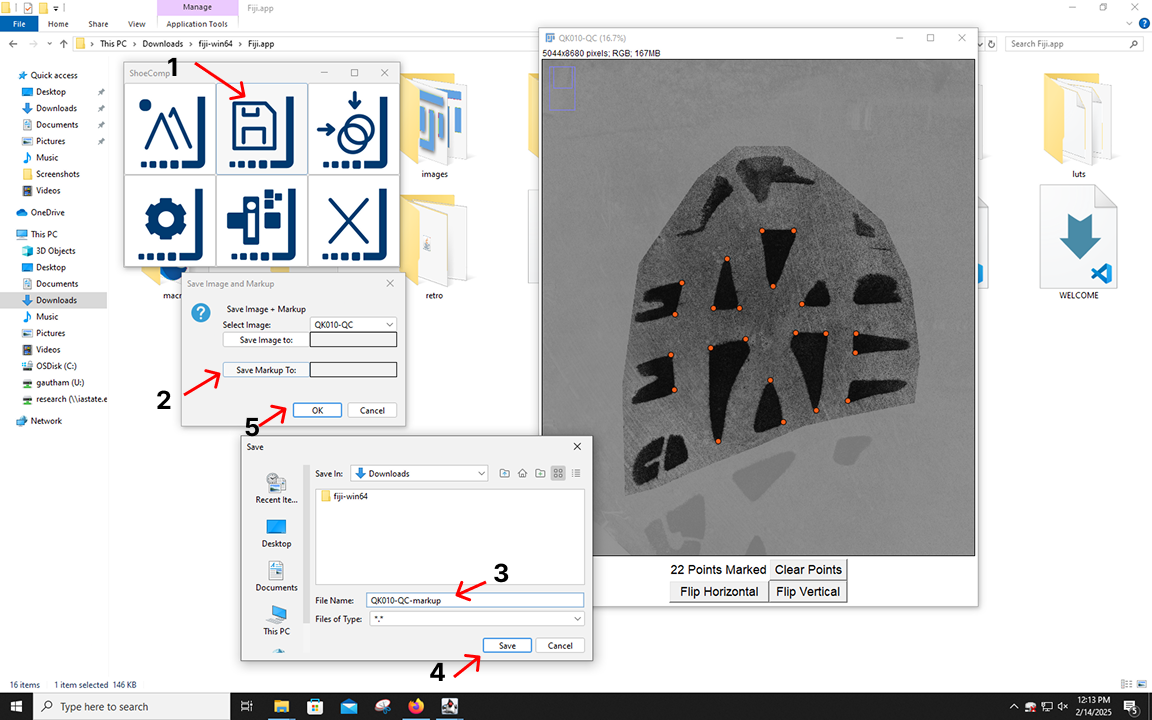
\includegraphics[width=0.8\linewidth]{images/step_5a-anno.png}
	\end{center}
	\caption{Saving your markup as JSON. Click on \texttt{Save Markup}, then \texttt{Save
			Markup To:}, then write a filename to save, click \texttt{Save}, and then click
		\texttt{OK}. You can also save the cropped image if necessary.}
	\label{fig:step5a}
\end{figure}

Once the markup has been saved, you can close the application or just the window. When
reloading the image, you can use the saved JSON markup later to resume your work:

\begin{figure}[H]
	\begin{center}
		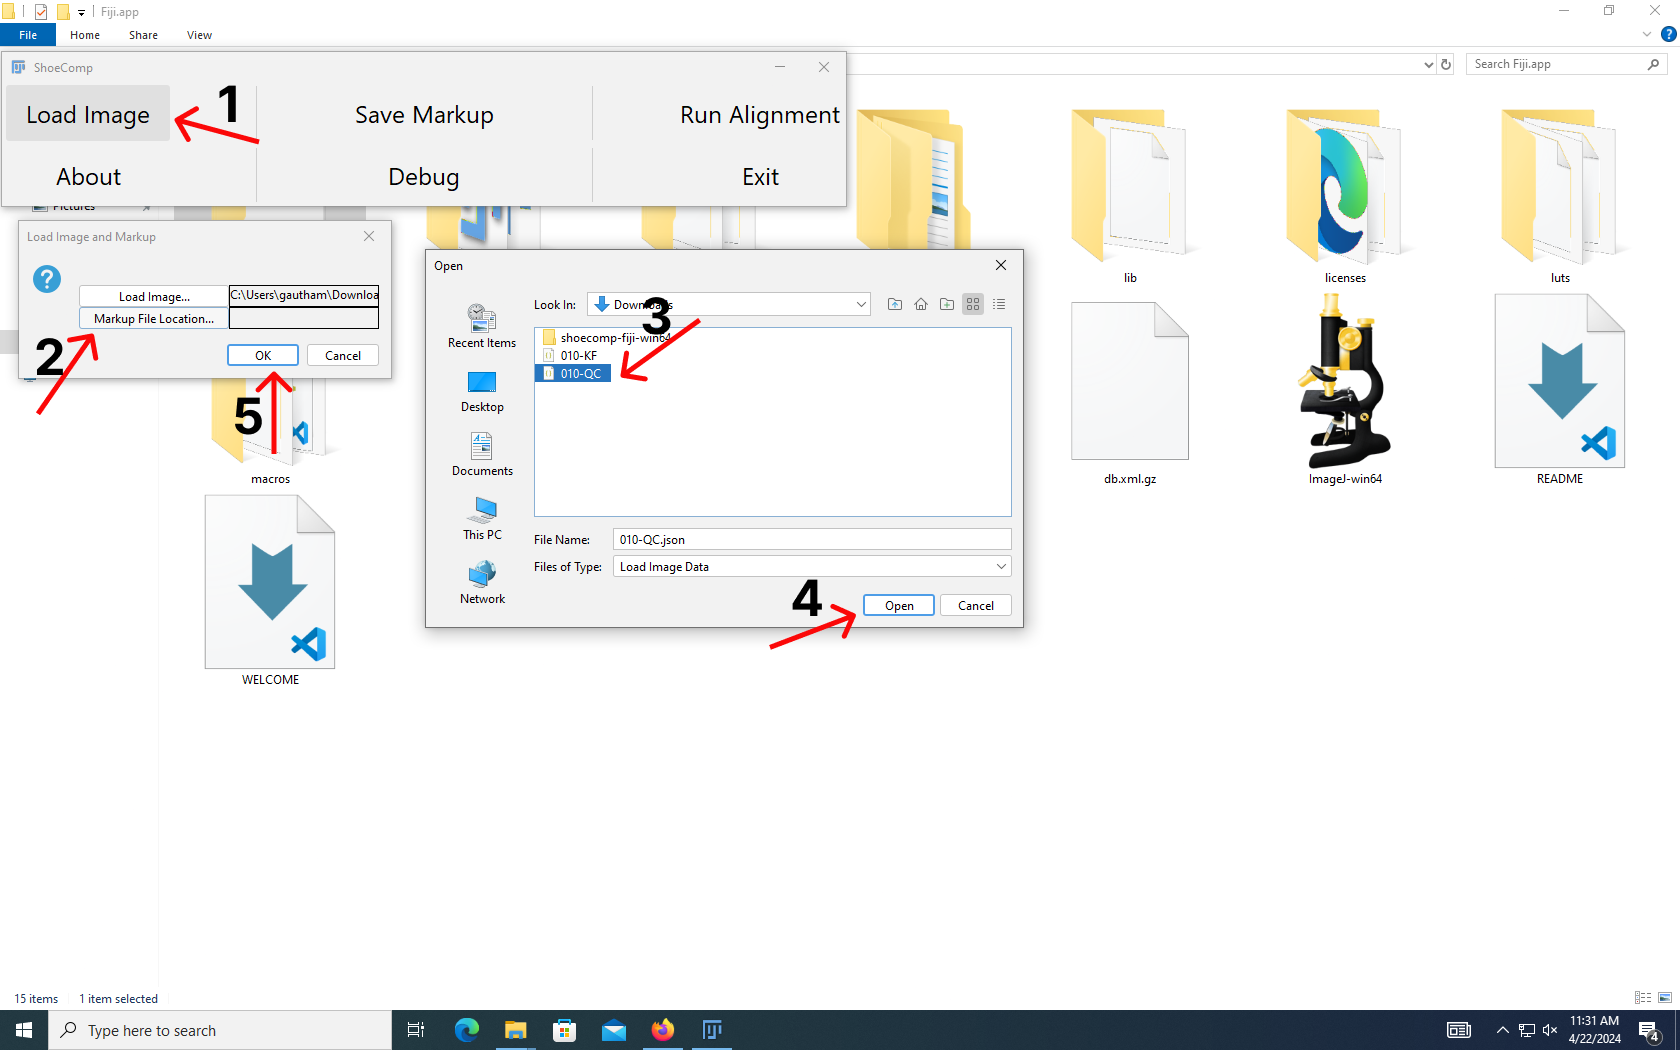
\includegraphics[width=0.8\linewidth]{images/step_5b-anno.png}
	\end{center}
	\caption{When re-loading the image similar to \autoref{fig:step4a}, you can now click on \texttt{Markup File Location} and load the JSON file to resume with your previously loaded markup.}
	\label{fig:step5b}
\end{figure}

\section{Aligning Marked Images}%

Now, let's suppose we have marked up the two images \texttt{QK010-QC.JPG} and
\texttt{QK010-KF.JPG} as below. To obtain an alignment, we hope that the marked points are
reasonably accurate, and that a decent number of points (at least 3 points) are common
between both images.

\begin{figure}[H]
	\begin{center}
		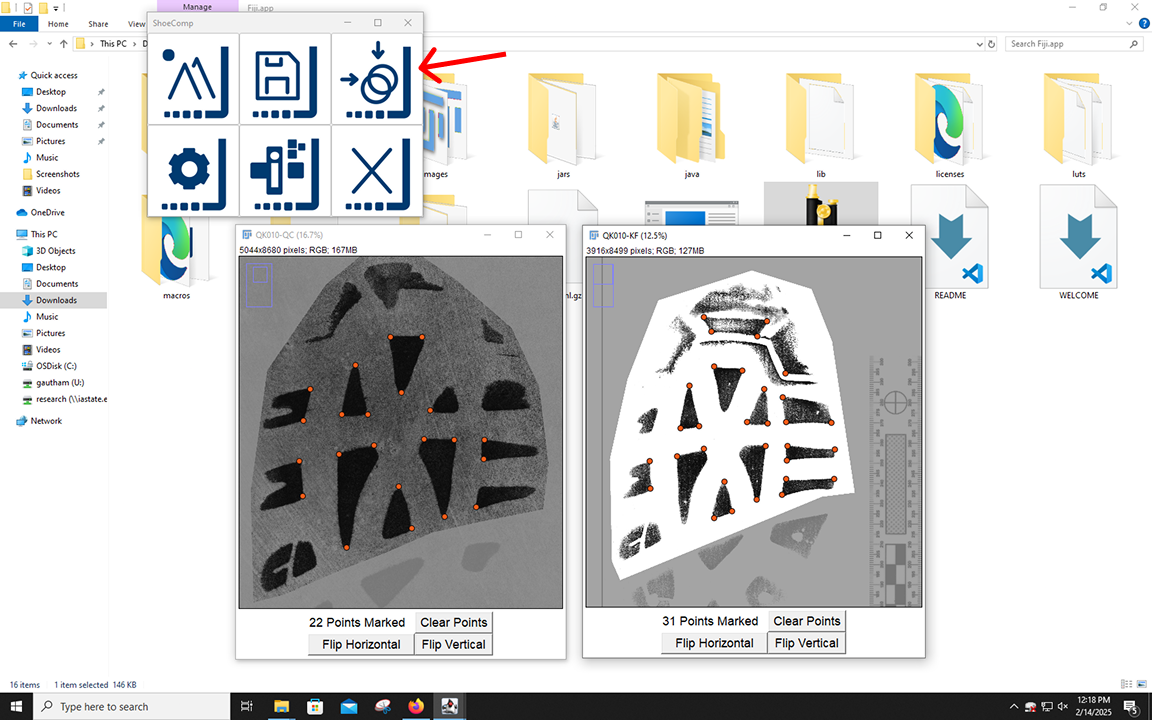
\includegraphics[width=0.8\linewidth]{images/step_6-anno.png}
	\end{center}
	\caption{We have marked around 20-30 points in both images, and now we are ready to try the alignment algorithm.}
	\label{fig:step6}
\end{figure}

We would like to align these shoeprint images, obtain a visualization of how well these
images can be aligned, and also obtain some numerical scores that tell us how good the
alignment is. We can do that by clicking on the \texttt{Run Alignment} button:

\begin{figure}[H]
	\begin{center}
		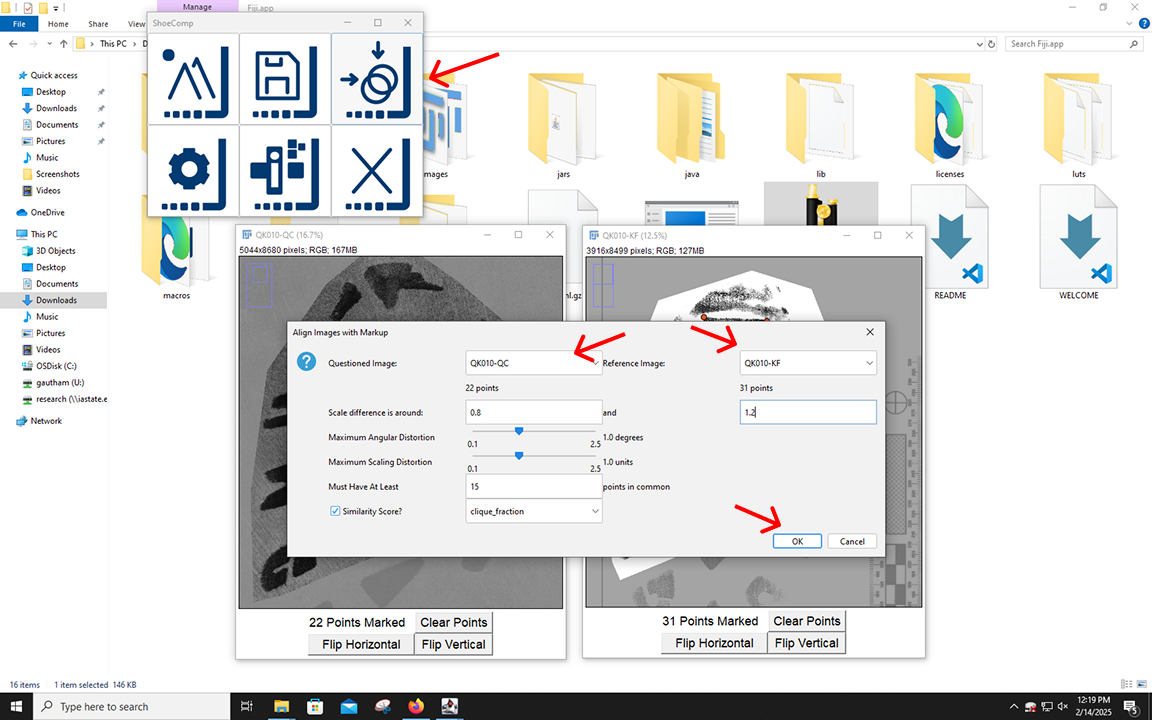
\includegraphics[width=0.8\linewidth]{images/step_8a-anno.png}
	\end{center}
	\caption{Align shoeprint images. Click on \texttt{Run Alignment}, select \texttt{QK010-QC} as the questioned image,
		\texttt{QK010-KF} as the reference image, fill an approximate range for scale difference
		between these images (it should be around 1 in this case). For now, let's use the defaults
		for the maximum allowed distortion, but generally smaller values indicate more rigid
		transformations. We would like the alignment to align at least 15 points in common from
		the points we marked. Finally, we select one of the similarity scores to view.}
	\label{fig:step8a}
\end{figure}
\vspace*{-1.5em}
The alignment might take some time to run, depending on the number of points marked and
how large the allowed ranges for scaling and distortion are.

\begin{figure}[H]
	\begin{center}
		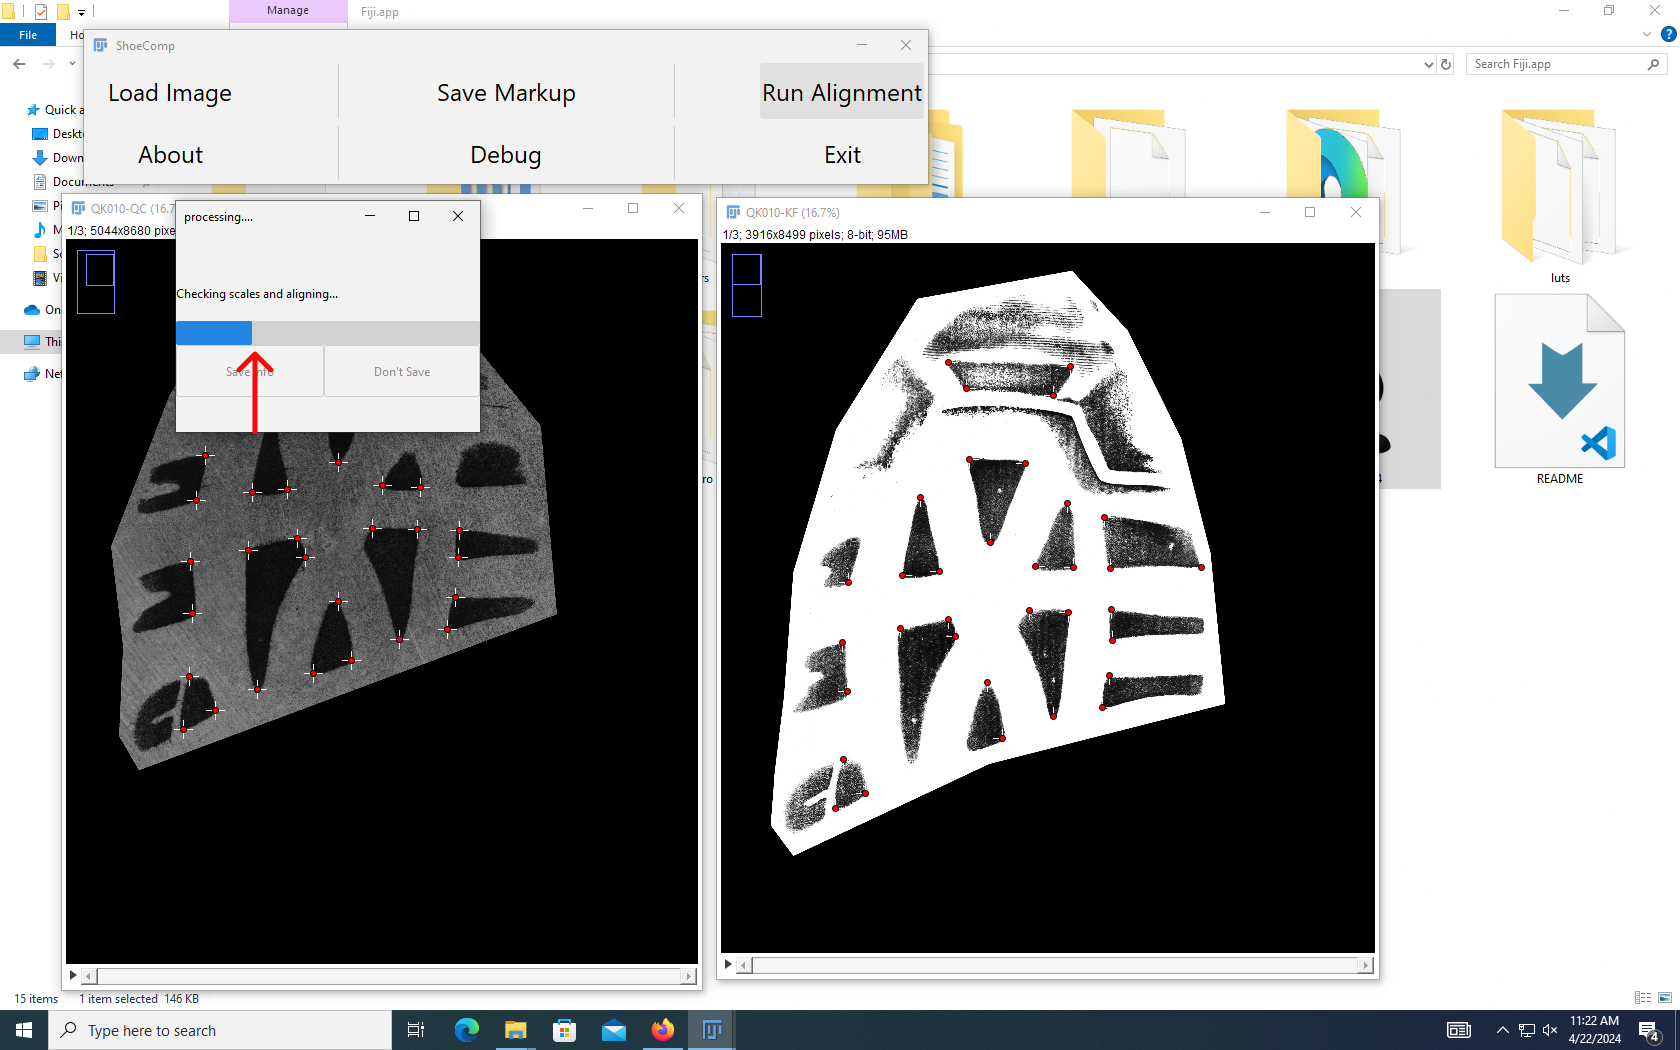
\includegraphics[width=0.8\linewidth]{images/step_8b-anno.png}
	\end{center}
	\caption{The alignment process is running, trying to resolve differences in rotation,
		translation, and scale.}
	\label{fig:step8b}
\end{figure}

Sometimes the alignment process may fail, which means you would have to mark more points,
allow for more distortion, or reduce the minimum number of points required for an
alignment.

\begin{figure}[H]
	\begin{center}
		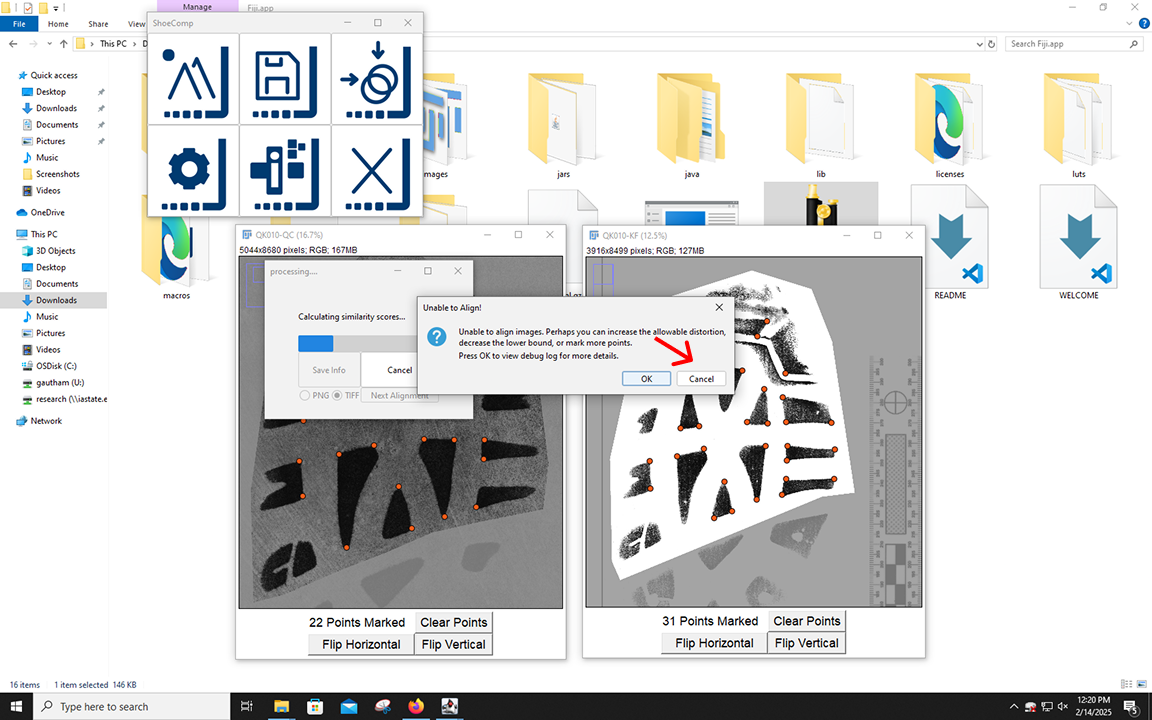
\includegraphics[width=0.8\linewidth]{images/step_8b_fail-anno.png}
	\end{center}
	\caption{Alignment process failed. Click cancel and try to align again.}
	\label{fig:step8b_fail}
\end{figure}

After the alignment process has successfully completed, we see two new windows: one
showing the overlay of the images, and the other showing a similarity score measurement
related to the alignment.

\begin{figure}[H]
	\begin{center}
		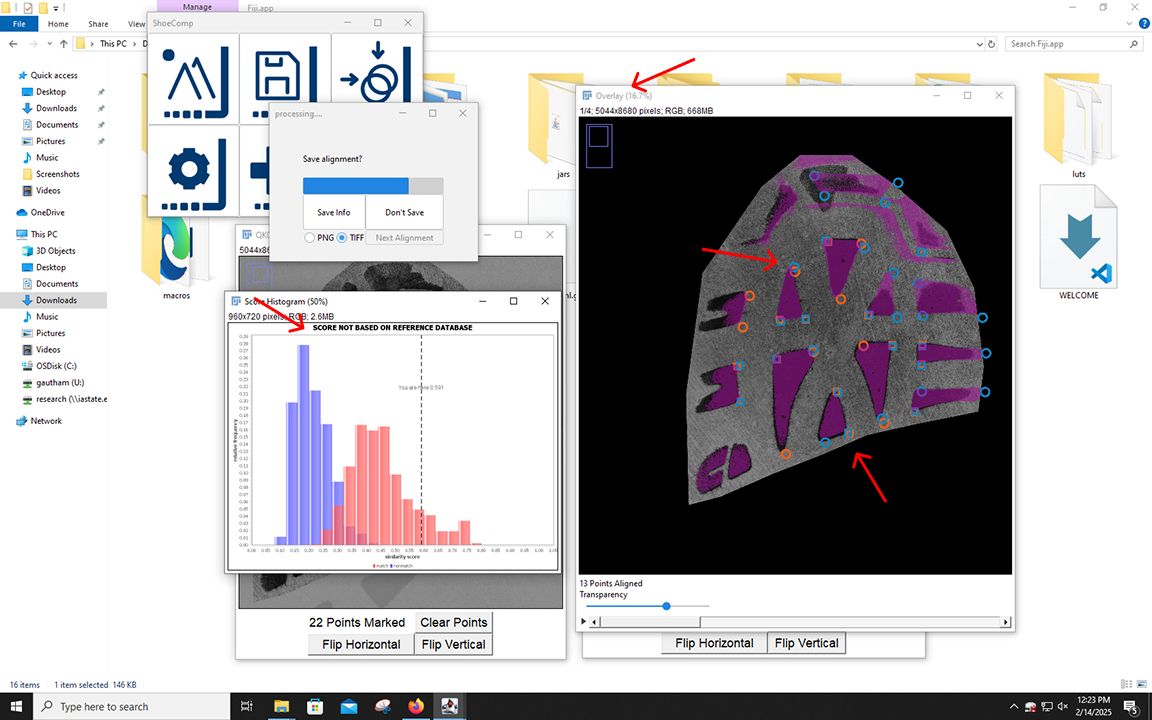
\includegraphics[width=0.8\linewidth]{images/step_8c-anno.png}
	\end{center}
	\caption{Alignment complete. You can look at the purple overlay and the points to see how well the reference image has been aligned to the questioned image. Square points indicate those points were selected in the alignment, and circular points indicate those points which were not. Generally, we would expect the square points to be almost on top of one another. The similarity score provides a numerical measurement with respect to an example background distribution.}
	\label{fig:step8c}
\end{figure}

If you'd like to find other possible alignments, you can click \texttt{Next Alignment} if
possible. To retry the alignment, you can click \texttt{Don't Save} and try again.
However, this alignment seems to be the only one satisfying our constraints, so let's
click on \texttt{Save Info}:

\begin{figure}[H]
	\begin{center}
		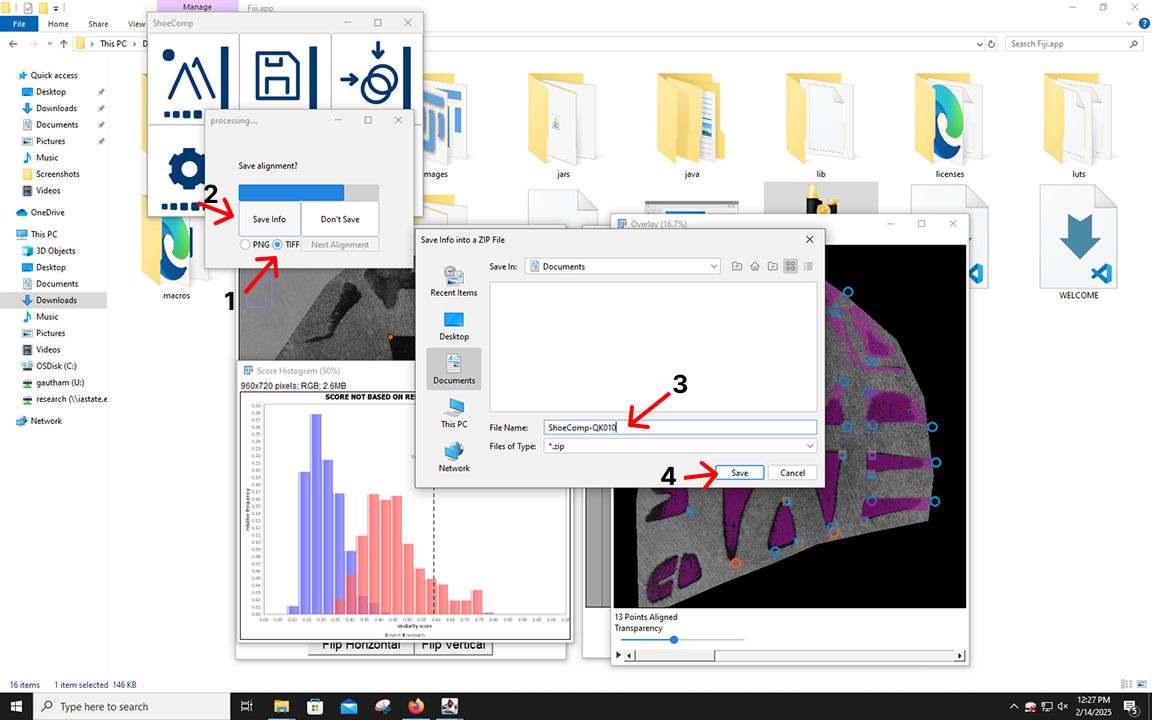
\includegraphics[width=0.8\linewidth]{images/step_8d-anno.png}
	\end{center}
	\caption{Saving the alignment into a ZIP file. Select image format as PNG or TIFF, Click on \texttt{Save Info}, and write the filename of ZIP file into which the alignment will be saved, and then click \texttt{Save}.}
	\label{fig:step8d}
\end{figure}

Once the ZIP file has been saved, you can open it to view the components of the alignment
process. The ZIP file at present contains:

\begin{itemize}
	\item three JSON files: one for each image markup, and one for the points calculated
	      during the alignment,
	\item three PNG/TIFF files corresponding to the questioned image: the original image, the
	      polygon mask indicating the relevant region, and the points marked.
	\item three PNG/TIFF files corresponding to the reference image: the original image, the
	      polygon mask indicating the relevant region, and the points marked.
	\item three PNG/TIFF files corresponding to the reference image, \textit{transformed so
		      that they align to the questioned image}: the original image, the
	      polygon mask indicating the relevant region, and the points marked.
\end{itemize}

The TIFF images can be overlaid in software like Photoshop to obtain something like the
purple overlay for use in a report. In the future, the entire ZIP file can be submitted
for further processing and calculation of more similarity scores.

\begin{figure}[H]
	\begin{center}
		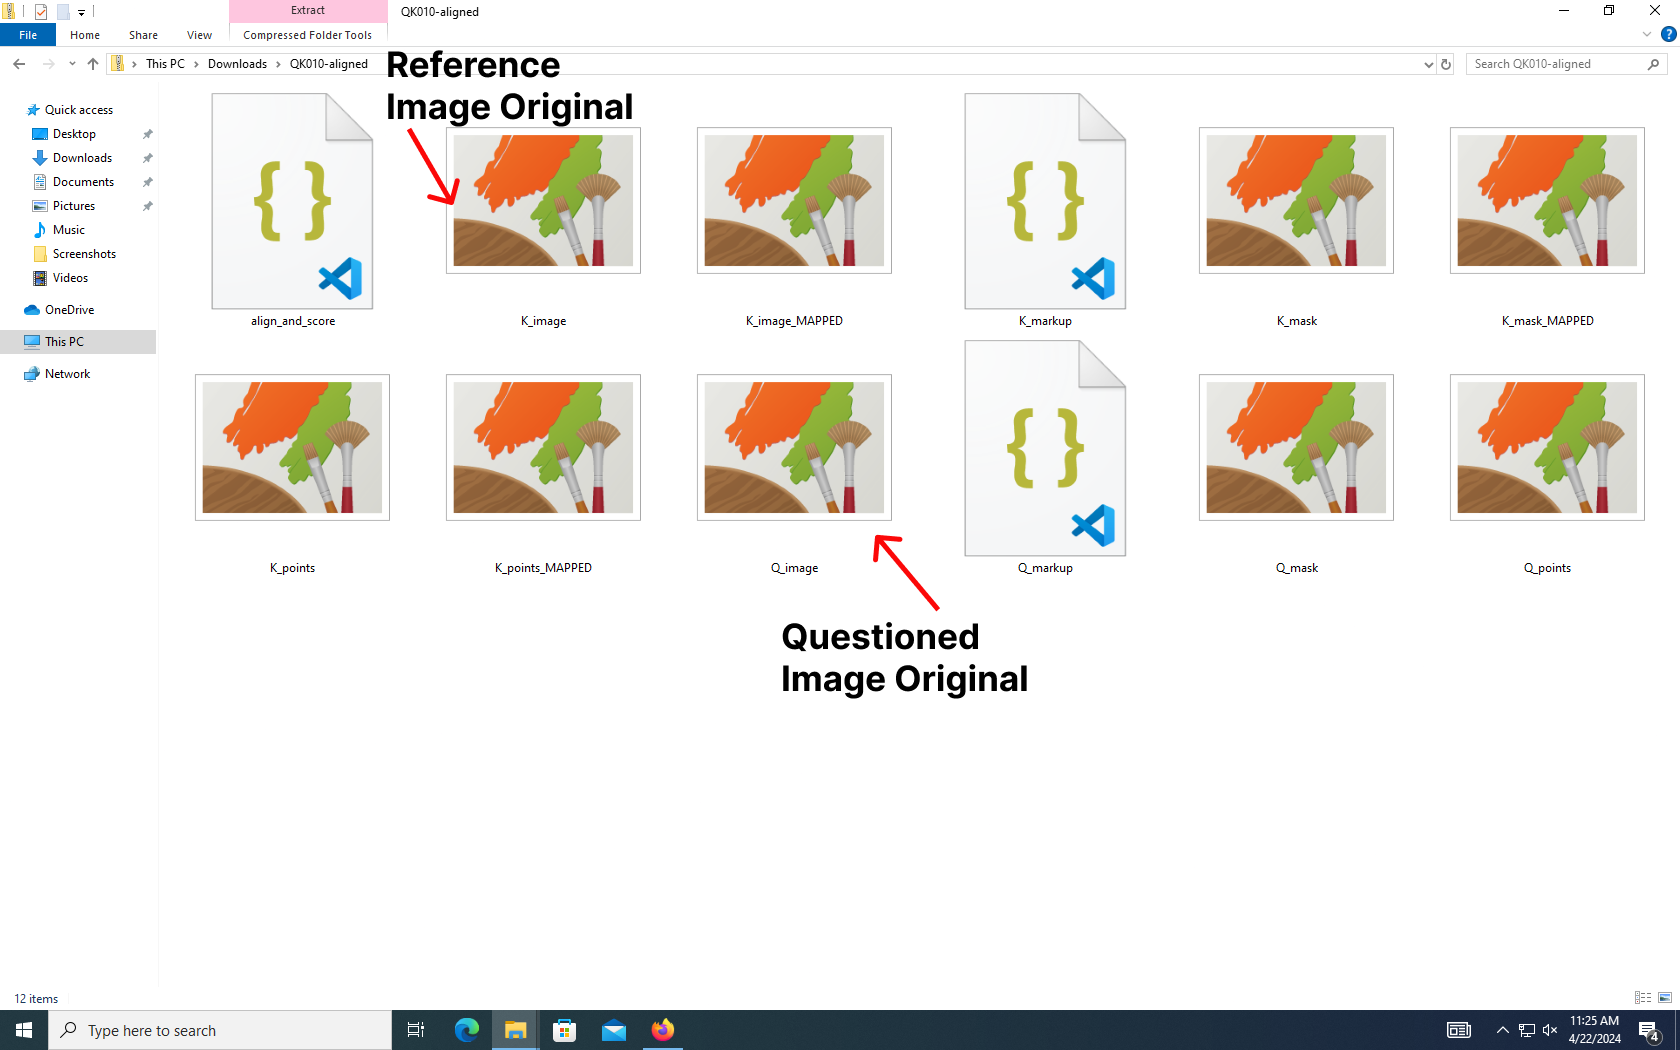
\includegraphics[width=0.8\linewidth]{images/step_10-anno.png}
	\end{center}
	\caption{The components of the saved ZIP file, indicating a completed alignment.}
	\label{fig:step10}
\end{figure}

\newpage
\chapter{Summary and Future Work}%

This document provides a user guide to ShoeComp, a shoeprint markup and alignment tool
developed by CSAFE at Iowa State University. The Java-based tool provides a simple user
interface to mark interest points on shoeprints, and aligns them using a maximum-clique
based method that handles rotation, translation, scale, and a bit of distortion as well.
The user can view an overlay of the alignment, and save the aligned images for use in
reports, or submit them for further similarity calculations.

\section{Updating ShoeComp}

By default, ShoeComp does not need to connect to the internet to run any updates, and we
would prefer to avoid automatic/background internet connections. However, it may sometimes
run a local check at startup to confirm all the libraries are available. This check at
startup is harmless -- you can close the complaining windows if any appear. We hope figure
out the relevant code causing this automatic check, and disable it soon. \\

To update ShoeComp, you can just delete the relevant ZIP file and folders, and download a
new one from the latest release on Github: \selfref{https://github.com/CSAFE-ISU/shoecomp}
\\

Future improvements for ShoeComp include: adding more similarity scores and visualizations,
checking for multiple possible optimal alignments, enabling polynomial/thin-plate-spline
alignment transformations, creating a smoother user interface, and of course, fixing
errors in the code. Let us know what you'd like to see:
\selfref{https://forensicstats.org}

\section{Performance Considerations}

The alignment algorithm might take a bit of time if you have more than 30 points marked in
each image. The speed of the algorithm is connected to:

\begin{itemize}
	\item Number of points marked in each image: around 30 is good, but more points means
	      a lot slower. At present, there doesn't seem to be a way around this, but we might find
	      better approximation algorithms.
	\item The allowable scale range: the default range is $0.8$ to $1.2$. We recommend
	      picking scale range of $\frac{1}{N}$ to $N$, but larger ranges will slow down the
	      algorithm a bit.
	\item Maximum allowed distortion: the more distortion you allow, the slower the
	      algorithm will be. At present, we recommend around 0.5 to 5 degrees of angular
	      distortion at most, and around 0.1 to 1 units of scaling distortion at most.
	\item Lower bound of common points: the minimum number of points the alignment should
	      have to be considered valid. Keeping a high lower bound means the algorithm will
	      run faster, but it might also not find any alignments that are so good.
\end{itemize}

\newpage
\nocite{*}
\bibliography{refs.bib}

\end{document}
